\documentclass{article}

\usepackage{fancyhdr} % Required for custom headers
%\usepackage{lastpage} % Required to determine the last page for the footer
\usepackage{extramarks} % Required for headers and footers
\usepackage[usenames,dvipsnames]{color} % Required for custom colors
\usepackage{graphicx} % Required to insert images
\usepackage{listings} % Required for insertion of code
\usepackage{courier} % Required for the courier font
\usepackage{amsmath, mathtools} %Required for math stuff
\usepackage{amssymb}
\usepackage{graphicx} % Required for including figures
\usepackage{siunitx}
\usepackage{cancel}
\usepackage{empheq}
\usepackage{tcolorbox}
\usepackage{bm}
\usepackage{float}
\usepackage{subcaption}

% Margins
\topmargin=-0.45in
\evensidemargin=0in
\oddsidemargin=0in
\textwidth=6.5in
\textheight=9.0in
\headsep=0.25in

\linespread{1.1} % Line spacing

% Set up the header and footer
\pagestyle{fancy}
\lhead{\Name} % Top left header
\chead{\Title} % Top center head
\rhead{\Date} % Top right header
\lfoot{\lastxmark} % Bottom left footer
\cfoot{} % Bottom center footer
%\rfoot{Page\ \thepage\ of\ \protect\pageref{LastPage}} % Bottom right footer
\renewcommand\headrulewidth{0.4pt} % Size of the header rule
%\renewcommand\footrulewidth{0.4pt} % Size of the footer rule

\setlength\parindent{0pt} % Removes all indentation from paragraphs

%----------------------------------------------------------------------------------------
%	NAME AND CLASS SECTION
%----------------------------------------------------------------------------------------

\newcommand{\Title}{DMDc Update} % Title of the set of notes
\newcommand{\Date}{} % Today's date
\newcommand{\Class}{} % Course/class
\newcommand{\ClassInstructor}{} % Teacher/lecturer
\newcommand{\Name}{Anthony Corso} % Your name
\newcommand{\hl}{\noindent\makebox[\linewidth]{\rule{\linewidth}{0.4pt}}}

\begin{document}

\section*{What works}
I've have shown that DMDc works for suppressing vortex shedding in a very narrow set of circumstances (see fig \ref{fig:dmdc_working}). Namely, when the dynamics and control matrices ($A$ and $B$) are computed from snapshots taken from the proportional control of the same system. In this case, the DMDc + MPC algorithm creates essentially the same control policy.


\begin{figure}
  \centering
  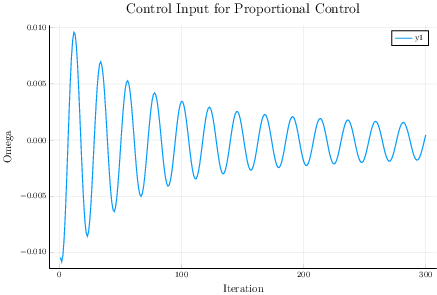
\includegraphics[scale=0.5]{../images/training_data.png}
  \caption{Control policy for the training data. The control policy comes from a proportional controller measuring the y-velocity at a point in the wake}
  \label{fig:training_data}
\end{figure}

% Figure that shows vortex shedding suppression
\begin{figure}
  \centering
  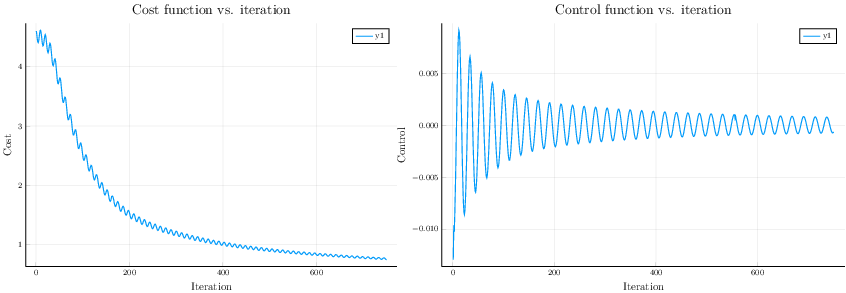
\includegraphics[scale=0.5]{../images/dmdc_working.png}
  \caption{Control policy from DMDc dynamics with MPC controller.}
  \label{fig:dmdc_working}
\end{figure}


I think this can be regarded as a minor success since the DMDc policy was entirely determined from MPC on the dynamical model that DMDc had constructed. But, as will be shown in the next section, this dynamical model is appears to be fragile and doesn't work in most other circumstances.

\section*{What Doesn't work}
When $A$ and $B$ are found from training data that deviates even slightly from the proportional control data, MPC doesn't seem to work at all. I have tracked this back to the fact that the predictive capabilities of DMDc seem to fail outside of the specific circumstances of the training data.

In order to evaluate the predictive capabilities of DMDc, I did the following:
From a sample MPC run, I copied the dynamics matrices, $A$ and $B$, the projection matrix $U$, and all of the simulation data from the run. Then for each iteration of the simulation run, the following 16 timesteps are predicted using the dynamical system. If the $t^{\rm th}$ frame of the simulation is flattened into a state vector $x_t$, and the control input is $u_t$, then we predict via
\begin{align*}
\tilde{x}_t &= U^T x_t \\
\tilde{x}^{\rm pred}_{t+1} &= A \tilde{x}_t + B u_t \\
x^{\rm pred}_{t+1} &= U \tilde{x}^{\rm pred}_{t+1}
\end{align*}

Then at each predicted timestep, the error in the prediction can be found via the norm $|| x^{\rm pred}_{t} - x_t ||$, where $x_t$ is the exact state, found from the simulation.



% Figure that shoes the predictive power to a dmdc decomposition
\begin{figure}
  \centering
  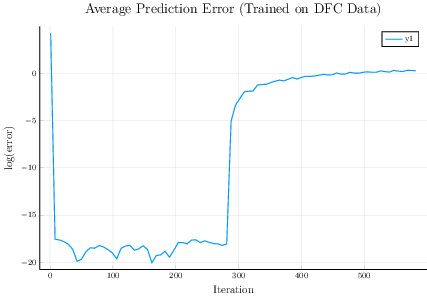
\includegraphics[scale=0.5]{../images/pred_error_working}
  \caption{The prediction error of the DMDc model trained from the proportional control data, predicting the proportional control data}
  \label{fig:pred_error_working}
\end{figure}

\begin{figure}
  \centering
  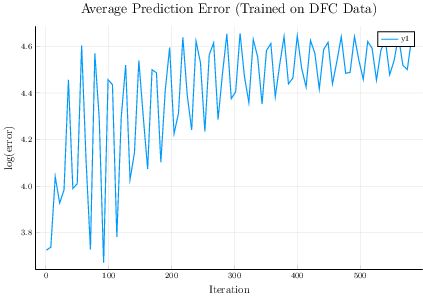
\includegraphics[scale=0.5]{../images/pred_error_not_working}
  \caption{The prediction error of the DMDc model trained from a deep flow control data set, predicting the proportional control data}
  \label{fig:pred_error_working}
\end{figure}

\section*{Things I've tried}

\begin{itemize}
  \item Used many different types of input training data and checked the predictive power on many other sets of data
  \item tried online computation of the $A$ and $B$ matrices, for each timestep, or every interval of 20 timesteps. Due to the sensitivy of DMDs capbility of predicting future dynamics, the constant recomputing of these matrices seems to cause the algorithm to become unstable and fail
\end{itemize}

\end{document}
